\subsubsection*{Live Coding for Uncertainty
  Quantification}

The ability to stop, modify, or restart computations `in flight' has
the potential to significantly improve the efficiency of an
uncertainty analysis. There exist many algorithms, for example
adaptive Markov chain Monte Carlo methods~\parencite{GilksEtal1994}, 
which attempt to choose the best samples based on the sampling
history. For complex problems however, a domain expert
may often have
a better idea about the region of the parameter domain where function
evaluations should be concentrated. Through live programming within a
tight feedback loop a domain expert can incrementally guide the
current sampling strategy being used for uncertainty 
quantification, and in turn be guided by 
real time information derived from the reduced order model 
(such as surpluses
provided by sparse grid approximation to 
identify important parameter dimensions and regions of interest), 
to improve the end result. The resulting strategies are expected to be
more aggressive in nature as they are better targeted to the specific
problem at hand. The result of this is more efficient quantification of
uncertainty.

In this project, using live coding to accelerate the feedback loop between
$\mathbf{p}$ and $Q(U_{\mathbf{p}})$, together with estimates of its
uncertainty,  will give a scientist the ability to interactively
\emph{explore} the connection (and the associated uncertainty) between
the different dimensions of $\mathbf{p}$ and the overall response of
the system. This will be used to {\bf rapidly prototype software} with a view to 
identifying the necessary interactive controls needed to modify and interact with 
the final, relased and running, software in real-time. 
By understanding the human-factors and systems-level time
constraints on the delivery of useful information in disaster-response
settings, we will also be able to specify timing requirements on our model
simulations as in the next section. 
%By developing software that is time-constrained and
%time-aware, we will be able to provide decision makers with
%information when it is needed and with an estimate on the uncertainty
%of that information.
%Ultimately, the scientist needs an \textbf{interactive interface} for
%gleaning insights from their models in the presence of these
%challenges.
%\newpage

%\begin{figure}
 % \centering
  %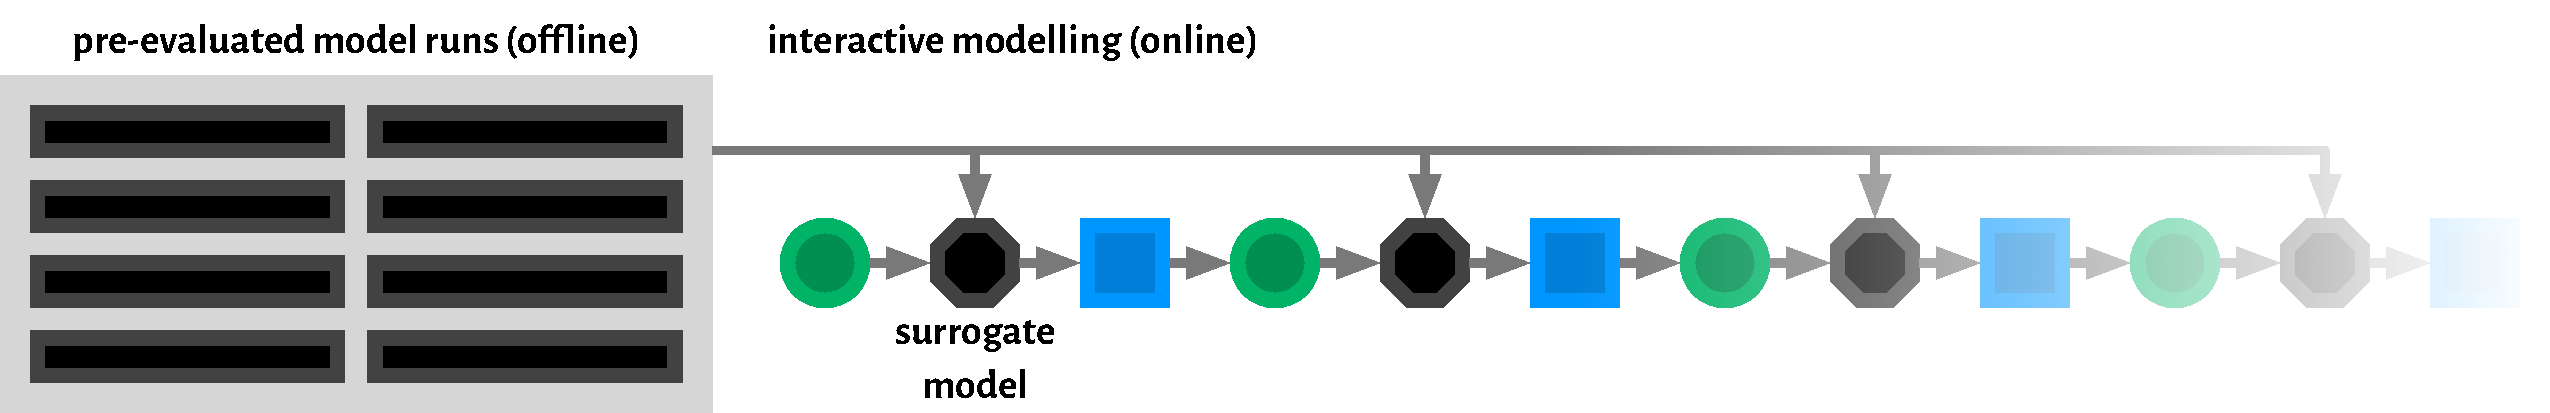
\includegraphics[width=\textwidth]{figures/sg-surrogate-model-fb-loop.pdf}
  %\caption{Using the sparse grids and reduced basis models, the computationally
   % expensive model calculations can be done ahead-of-time and used to
    %construct a surrogate model which can be used to re-claim the
    %interactive workflow of Figure~\ref{fig:unrolled-fb-loop}}.
  %\label{fig:sg-surrogate-model-fb-loop}
%\end{figure}

%Impact: new algorithms, software, high performance computer systems
%and visualisation techniques for time-bound environmental simulation
%with uncertainty. New software tools for the simulation of flood
%surges and tsunami. New methodologies for rapid and agile software
%development and usability using live programming. New knowledge of
%human-in-the-loop requirements for support systems in the context of
%environmental disaster management. New algorithms, software, high
%performance computer systems and visualisation techniques for
%time-bound environmental simulation with uncertainty. New software
%tools for the simulation of flood surges and tsunami. New
%methodologies for rapid and agile software development and usability
%using live programming. New knowledge of human-in-the-loop
%requirements for support systems in the context of environmental
%disaster management.


